\documentclass[a4paper,11pt,spanish]{article}

\textwidth 18.5cm
\textheight 26cm
\topmargin -2cm
\oddsidemargin -1.5cm
\parskip .3em
\parindent 0cm

%your favourite packages here
\usepackage[spanish]{babel}
% \usepackage{lineno}
% \usepackage{mathptmx}
%\usepackage{psfrag,graphicx}
\usepackage{amsmath}
\usepackage{amssymb}
\usepackage{amsfonts}
\usepackage{bm}
%\usepackage{bbm}
\usepackage{color}
\usepackage{latexsym}
\usepackage{epstopdf}
\usepackage{color}
%\usepackage{times}

\usepackage{psfrag,graphicx}
%\usepackage{picins}
\usepackage{natbib}
\usepackage{epstopdf}\DeclareGraphicsRule{.tif}{png}{.png}{`convert #1 `basename
#1 .tif`.png}
%\usepackage{dsfont}
%\usepackage{mathtools}

\definecolor{mygrey}{gray}{0.35}
\definecolor{myblue}{rgb}{0.2,0.2,0.8}
\definecolor{myzard}{cmyk}{0,0,0.05,0}
\definecolor{mywhite}{rgb}{1,1,1}
\definecolor{myred}{rgb}{1,0.,0.3}

\def \barl {\begin{array}{rl}}
\def \ea {\end{array}}
%\definecolor{myblue}{named}{MidnightBlue}
\usepackage[colorlinks=true,citecolor=myblue,linkcolor=myred]{hyperref}
\def\beq{\begin{equation}}
\def\eeq{\end{equation}}
\def\ba{\begin{align}}
\def\enda{\end{align}}
\def\bi{\begin{itemize}}
\def\ei{\end{itemize}}
\def\bs#1{\boldsymbol{#1}}
\def\txt#1{\textrm{#1}}

\newcommand{\eq}[1]{Eq.\;(\ref{#1})}

\newcommand{\sgn}{\operatorname{sgn}}
\def\C{{\mathbb{C}}} \def\F{{\mathbb{F}}}
\def\N{{\mathbb{N}}} \def\Q{{\mathbb{Q}}}
\def\R{{\mathbb{R}}} \def\Z{{\mathbb{Z}}}
\def\cH{{\mathcal H}}
\def\bfsigma{\boldsymbol{\sigma}}
\def\bfmu{\boldsymbol{\mu}}
\def\dd{\mathord{\rm d}} \def\Det{\mathop{\rm Det}}
\def\dist{\mathop{\rm dist}} \def\ee{\mathord{\rm e}}
\def\End{\mathord{\rm End}} \def\ev{\mathord{\rm ev}}
\def\id{\mathord{\rm id}} \def\ii{\mathord{\rm i}}
\def\min{\mathord{\rm min}} \def\mod{\mathord{\rm mod}}
\def\prob{\mathord{\rm prob}}
\def\tr{\mathop{\rm Tr}}
\def\half{\textstyle\frac{1}{2}}
\def\third{\textstyle\frac{1}{3}}
\def\fourth{\textstyle\frac{1}{4}}

\graphicspath{{figs/}}

\newcommand{\da}{\downarrow}
\newcommand{\ua}{\uparrow}

\renewcommand{\ii}{{\rm i}}
\renewcommand{\ee}{{\rm e}}

%brackets
 \newcommand{\ket}[1]{|#1\rangle}
 \newcommand{\bra}[1]{\langle #1|}
 \newcommand{\braket}[2]{\langle #1|#2\rangle}

 \newcommand{\ketbra}[2]{\ket{#1}\bra{#2}}
 \newcommand{\proj}[1]{\ketbra {#1}{#1}}
 \newcommand{\biket}[2]{\ket{#1\;#2}}
 \newcommand{\bibra}[2]{\bra{#1\;#2}}
 %\newcommand{\ketbradif}[2]{\biket {#1}{#2}\bibra {#1}{#2}}
 \newcommand{\preespacio}{\!\text{\hspace{0.2 ex}}}
 \newcommand{\postespacio}{\!\text{\hspace{0.75 ex}}}


 \begin{document}

\noindent{\large \bf Procesamiento Cu\'antico de la Informaci\'on - C. Cormick, FING - 1er sem. 2025}\\

\noindent{\large \bf Práctico 7 - Alternativas al modelo de circuitos}\\

\vspace{10pt}

\noindent{\bf Parte 1 - Computaci\'on cu\'antica adiab\'atica}

\begin{enumerate}
\item Considerar un qubit almacenado en alg\'un sistema f\'isico, por ejemplo un \'atomo. Suponemos que cada estado de la base computacional corresponde a un autoestado del operador Hamiltoniano, pero cada uno con una energ\'ia diferente, de manera que $H$ (en el subespacio que nos interesa) se escribe en la forma $H=E_0 \proj{0}+E_1\proj{1}$ con $E_0< E_1$. La probabilidad de medir el qubit y hallarlo en 0 es la misma que la probabilidad de medir el valor $E_0$ al medir la energ\'ia.

\begin{enumerate}
 \item Suponer ahora que tenemos dos de estos qubits, cada uno en un \'atomo diferente. Si estos dos \'atomos no tienen ninguna interacci\'on entre ellos, el Hamiltoniano total es la suma de los Hamiltonianos independientes, es decir $H_{\rm tot} = H_1\otimes \mathbb{I}_2+ \mathbb{I}_1 \otimes H_2$ (el $H$ del \'atomo 1 se asume igual al del 2, los sub\'indices indican sobre qu\'e subsistema act\'ua cada matriz). Escribir una base para el sistema compuesto, y escribir la forma matricial de $H_{\rm tot}$ en esa base. Indicar cu\'ales son entonces los posibles resultados en una medici\'on de la energ\'ia.

 \item Generalizar al caso de $n$ qubits todos iguales (\textexclamdown pero sin escribir la matriz!). Indicar cu\'al ser\'a la menor energ\'ia posible del sistema, y cu\'al el autovector asociado.
\end{enumerate}
 
\item Volvamos al caso considerado en el problema anterior, pero con un solo qubit. Supongamos que tenemos un estado inicial $\ket{\psi(0)} = \alpha(0) \ket{0}+\beta(0) \ket{1}$. La evoluci\'on temporal est\'a dada por la ecuaci\'on de Schr\"odinger:
$$\frac{d}{dt} \ket{\psi(t)} = - i \frac{H}{\hbar} \ket{\psi(t)}\,.$$ 
Escribiendo $\ket{\psi(t)}= \alpha(t) \ket{0}+\beta(t) \ket{1}$, usando las propiedades de la derivada y el hecho de que los kets $\ket{0}$, $\ket{1}$ son constantes, la ecuaci\'on de arriba es equivalente a un conjunto de dos ecuaciones lineales independientes, de la forma:
 $$\frac{d\alpha}{dt} = -i \frac{E_0}{\hbar} \alpha(t), \quad \frac{d\beta}{dt} = -i \frac{E_1}{\hbar} \beta(t)$$
La soluci\'on de esas ecuaciones es: 
$$\alpha(t) = e^{-iE_0 t/\hbar} \alpha(0), \quad \beta(t) = e^{-iE_1 t/\hbar} \beta(0)\,.$$


Considerar el siguiente caso particular: $E_0=0$, y $\alpha(0)=\beta(0)=1/\sqrt{2}$, o sea el estado inicial es el $\ket{+}$. Calcular cu\'anto tiempo tengo que esperar para que el estado se transforme en el $\ket{-}$.

\item Considerar el siguiente ejemplo en un sistema de 2 qubits: se tiene un Hamiltoniano inicial de la forma: $H_I = -(Z_1+Z_2)$, y un Hamiltoniano final de la forma: $H_F=Z_1 +Z_2-Z_1Z_2$. 
\begin{enumerate}
 \item Sabiendo que los autovectores de ambos Hamiltonianos son los de la base computacional, indicar cu\'ales son los autovalores correspondientes a cada estado para el instante inicial y el final. En particular indicar cu\'al es el estado de menor energ\'ia al principio y cu\'al al final.
 \item Suponer ahora que se tiene un Hamiltoniano que var\'ia en el tiempo seg\'un $H(t)= (t/T) H_F + (1-t/T) H_I$ con $t\in[0,T]$. Indicar los autovalores como funci\'on del tiempo y graficarlos. Mostrar que el m\'inimo valor del gap $\Delta(t)$ entre las dos energ\'ias m\'as bajas es cero y calcular a qu\'e tiempo $t$ se anula.
\end{enumerate}

\item Considerar un sistema de $n$ qubits con Hamiltoniano de la forma: $H=-\sum_{j=1}^n X_j$. Indicar el conjunto de sus autovalores, y en particular explicar cu\'al es el estado de menor energ\'ia.

\item Considerar un sistema de 2 qubits en el que el Hamiltoniano final es el $H_F$ del problema 3, mientras que el Hamiltoniano inicial es el del problema 4. Calcular num\'ericamente los autovalores de $H(t)= (t/T) H_F + (1-t/T) H_I$ con $t\in[0,T]$, graficar el gap como función de $t$, y ver que nunca se anula. Comparar con el gráfico del problema 3(b).

\end{enumerate}

\newpage

\noindent{\bf Parte 2 - Computaci\'on cu\'antica basada en la medici\'on}

% \vspace{10pt}

\begin{enumerate}\setcounter{enumi}{5}
\item Un ``estado grafo'' de n qubits se prepara en base a un grafo no-dirigido de n v\'ertices (cada v\'ertice identificado con un qubit) de acuerdo al siguiente procedimiento:
\begin{itemize}
 \item Preparar todos los qubits en $\ket{+}$.
 \item Aplicar compuertas $CZ$ entre todos los pares de qubits correspondientes a v\'ertices que son vecinos en el grafo (notar que todas las compuertas $CZ$ conmutan entre s\'i, as\'i que el orden de su aplicaci\'on da igual).
\end{itemize}

\begin{enumerate}
 \item Ver que si tengo un grafo inconexo, entonces el estado grafo va a ser un estado producto entre los grafos conexos que lo forman (en general, en este contexto suele estar impl\'icito que nos interesan los grafos conexos).
 \item Considerar el grafo formado por dos v\'ertices unidos. Escribir expl\'icitamente en notación de Dirac la forma del estado grafo asociado, y mostrar que es entrelazado. Indicar dos estabilizadores no triviales de ese estado.
\end{enumerate}

\item Dado un estado arbitrario de un qubit $\ket{\psi}=\alpha \ket{0}+\beta\ket{1}$, considerar los siguientes circuitos:
\begin{center}
 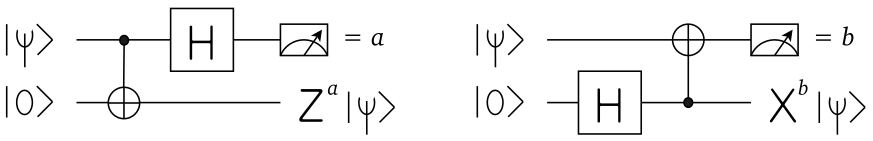
\includegraphics[width=250pt]{state_transfer.png}
\end{center}
En este contexto, $a,b\in\{0,1\}$ corresponden a los resultados de la medici\'on realizada sobre el primer qubit; es decir, el estado inicial del primer qubit se transfiere al segundo, a menos de un error de Pauli conocido que depende del resultado de la medici\'on. Para cada uno de los circuitos:

\begin{enumerate}
 \item Demostrar que el estado de salida del segundo qubit es efectivamente el indicado en el gráfico.
 \item Demostrar que las probabilidades para cada resultado al medir el primer qubit son iguales a 1/2.
% \item Usando el ítem anterior, escribir cómo sería la matriz densidad del segundo qubit si queremos representar el caso promedio, es decir si no usamos la información sobre cuál fue el resultado medido sino que consideramos ambas opciones con sus correspondientes probabilidades. Comparar con la matriz densidad que corresponde al estado final para cada uno de los resultados de la medición considerados individualmente. \textquestiondown A qué canal de ruido es equivalente el efecto del promediado?
\end{enumerate}


\item Demostrar, usando el problema anterior, que los circuitos de la izquierda tienen el efecto indicado (es decir que el estado final del segundo qubit es el que se indica en el gráfico). Además, usando propiedades conocidas de las compuertas, demostrar que los circuitos de la izquierda son equivalentes a los de la derecha:
\begin{center}
 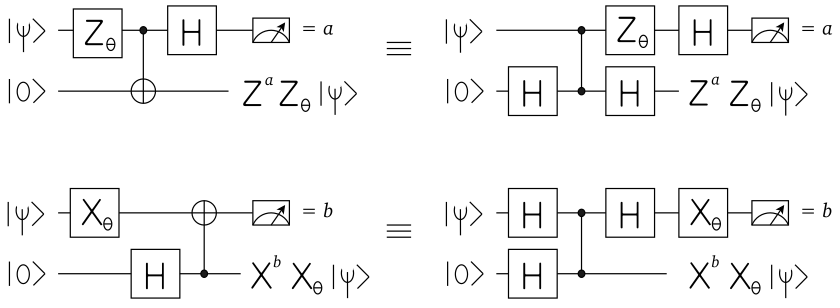
\includegraphics[width=300pt]{gate_transfer.png}
\end{center}
Aqu\'i, las compuertas involucradas se definen como: $X_\theta = \cos\theta\, \mathbb{I} - i\sin\theta X$, $Z_\theta = \cos\theta\, \mathbb{I} - i\sin\theta Z$. Lo que esto muestra es un modo de transferir al segundo qubit el estado obtenido luego de aplicar una compuerta $X_\theta$ o $Z_\theta$ sobre $\ket{\psi}$, a menos de un error de Pauli conocido que depende del resultado de la medici\'on.

\item {\it Opcional.} Inventarse un circuito muy simple de dos qubits, que contenga al menos una compuerta de un qubit y al menos una de dos qubits, y ver c\'omo ser\'ia su versi\'on equivalente en el modelo basado en la medici\'on. Implementar en el simulador IBM y chequear el resultado.

\end{enumerate}

\end{document}
